\documentclass[e4_tp2_main.tex]{subfiles}
\begin{document}
\newgeometry{top=2.5cm, bottom=2.0cm, left=2.25cm, right=2.25cm}

\section{Convertidor Boost para Lámpara LED de potencia}

\subsection*{LED's de Potencia: Efecto de la temperatura - Realimentación}
De la hoja de datos de OSRAM para el LUW-W5AP, se da la curva de $\Delta V(T)=V_F-V_F(25^{\circ})$, para la corriente $I_F$ máxima de 1400mA. La misma tiene pendiente negativa, es decir, que a mayor temperatura, la tensión en directa sobre el LED disminuye.

\begin{figure}[H]
\centering
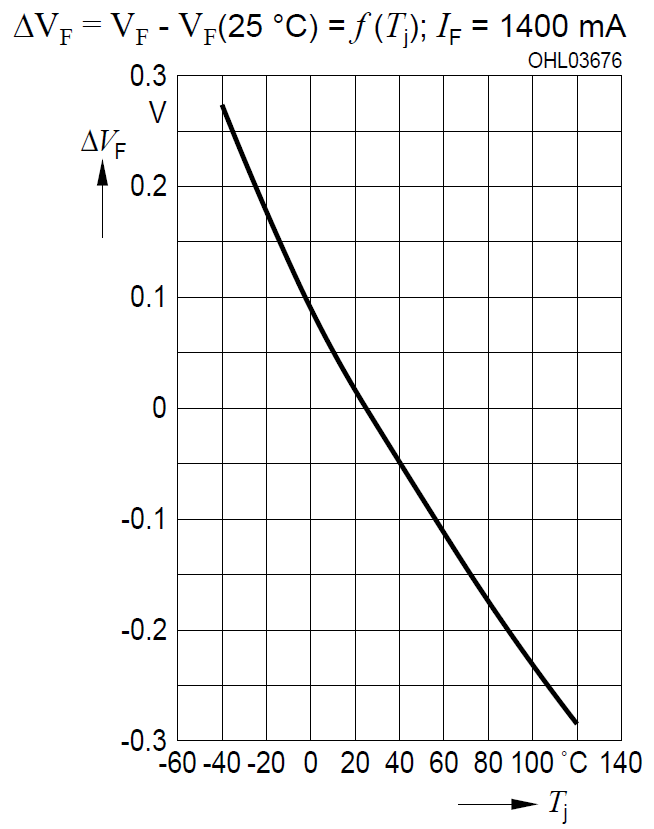
\includegraphics[width=0.3\linewidth]{Imagenes/Punto2/efectoT.png}
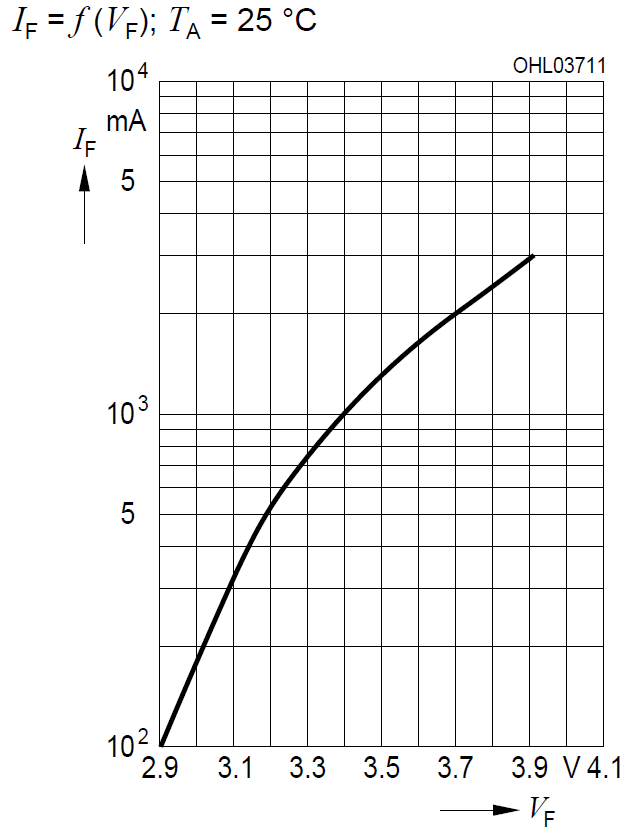
\includegraphics[width=0.29\linewidth]{Imagenes/Punto2/IF-VF.png}
\caption{Efecto de la temperatura en la $V_{LED}$: $\Delta V_F(T_j)$ - Curva de $I_F(V_F)$}
\end{figure}

Al trabajar con LED's de potencia, es conveniente realimentar la corriente en lugar de la tensión. Esto se debe a que si se produce una perturbación en la carga (es decir, para el caso de la simulación cortocircuitar dos LED's), si se está regulando tensión, caerá más tensión sobre los LED's restantes, por lo que la corriente aumentará, de acuerdo a la curva de $I_F(V_F)$ provista en la hoja de datos. Esto podría llevar a que los LED's se quemen por exceso de potencia.

\subsection*{LED's de Potencia: Variación del Brillo}
En el realimentador, el amplificador operacional amplifica la tensión sobre la resistencia sensora de la corriente ($R_2$), de manera de obtener a su salida la tensión de referencia de 2.5V para el LT1241. El lazo de realimentación ajusta la corriente para tener en el Pin 2 (FB) dicho valor de tensión dado que el operacional interno a la entrada se encuentra realimentado negativamente de forma externa con un RC entre su salida y el Pin 2 (que es la entrada inversora). Internamente, la entrada no inversora está a un potencial constante de 2.5V. Como el operacional realimentado negativamente busca llegar a que $V^+ = V^-$, de ahí obtenemos que la entrada del Pin 2 se lleva a 2.5V.\par
Teniendo esto en cuenta, Se busca en la hoja de datos el valor de corriente para el cual se obtiene la mitad del brillo (para el valor actual de 2A se obtiene el máximo). De acuerdo a la curva provista:

\begin{figure}[H]
\centering
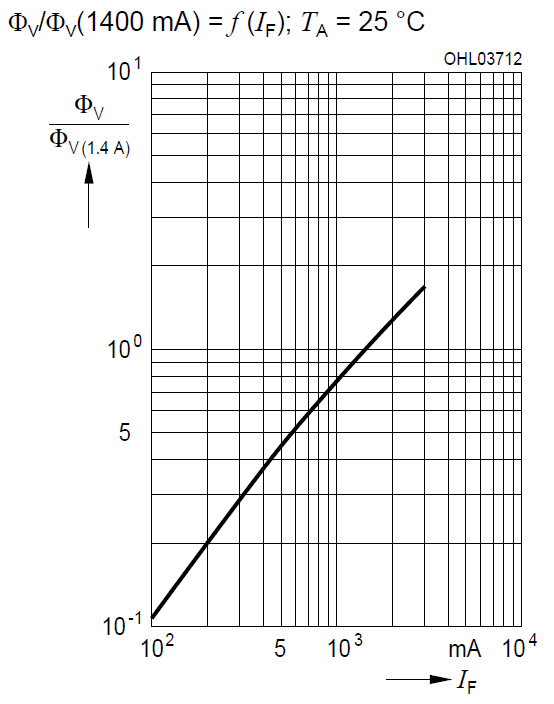
\includegraphics[width=0.3\linewidth]{Imagenes/Punto2/Lumen-IF.png}
\caption{Curva de $\frac{\Phi_V}{\Phi_V(1.4A)}(I_F)$}
\end{figure}

Se tiene que la mitad del brillo máximo se da a una corriente 
de 700mA. Por lo tanto, la tensión sobre la resistencia sensora $R_2$ será de: 

\[
I_F = 700mA \cdot 0.1\Omega = 0.07V
\]

Sabiendo que a la salida del operacional debe haber 2.5V, se despeja el nuevo valor para $R_6$:
\[
\frac{2.5V}{0.07V} = G = 35.7 \longrightarrow R_6 = 34.7K \Omega
\]

\subsection*{Oscilador - Frecuencia de Switching}
De la hoja de datos, en la sección de Oscilador, se indica que la frecuencia del LT1241 es el doble que la de switching. Entonces, para tener 75KHz, se buscará en la gráfica de $R_TC_T(f)$ el par de valores de componentes acordes para una frecuencia de 150KHz:

\begin{figure}[H]
\centering
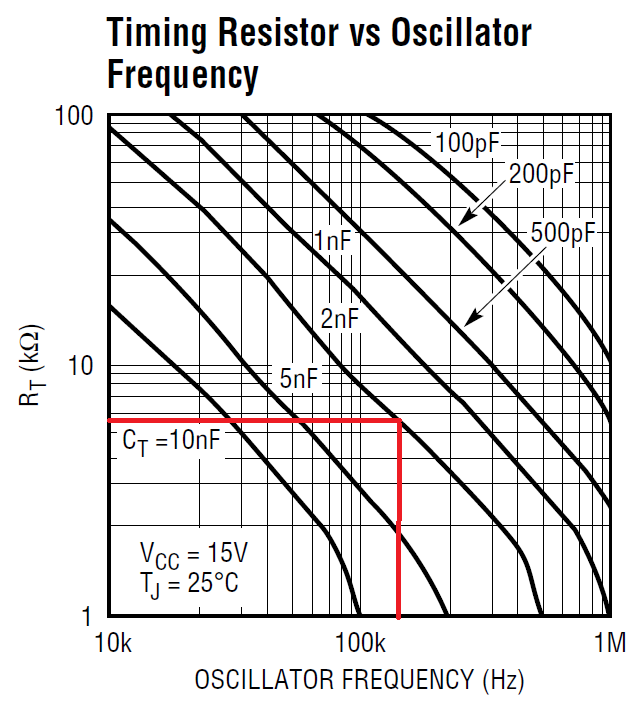
\includegraphics[width=0.3\linewidth]{Imagenes/Punto2/RT-OSC.png}
\caption{Curva de $R_TC_T(f)$}
\end{figure}

De donde se obtiene $R_T = 5.3K\Omega$ y $C_T = 2nF$. Es posible verificar mediante las ecuaciones provistas en la misma hoja:

\[
t_r = 0.583 \cdot R_T \cdot C_T \hspace{2cm} t_d = \frac{3.46 \cdot R_T \cdot C_T}{0.0164 \cdot R - 11.73}
\]
\[
T_{OSC} = t_r + t_d \longrightarrow f_{OSC} = 150KHz
\]
\[
f_{SW} = \frac{f_{OSC}}{2} = 75KHz
\]

\subsection*{$\mathbf{I_{PK}(I_O)}$ - Corriente pico en el switch en función de $\mathbf{I_O}$}
De la hoja de datos se tiene que, en general, la corriente pico en el switch es:

\[
I_{PK} = \frac{V_{Pin1} - 1.4V}{3R_S}
\]

Donde $R_S$ es la resistencia para el sensado de la corriente en el switch.

Tomando la sección de circuito de la hoja de datos, agregando la realimentación externa:

\begin{figure}[H]
\centering

\includegraphics[width=0.8\linewidth]{Imagenes/Punto2/IPK-Circuito.png}
\caption{Circuito para análisis de $I_{PK}$}
\end{figure}

Para la frecuencia de switching, se puede considerar el capacitor $C_3$ de baja reactancia, por lo que el circuito con el operacional se puede estudiar como un sumador.\par
Pasivando la entrada $V_{f}$, se tiene:

\[
V_{o1} = 2.5V \cdot \left(1+ \frac{10K}{10K}\right) = 5V 
\]

Pasivando la otra entrada fija de 2.5V:

\[
V_{o2} = V_{f} \cdot \left(- \frac{10K}{10K} \right) = -V_{f}
\]

Por lo que $V_{Pin1}$ resulta:

\[
V_{o} = V_{Pin1} = 5 - V_{f} = 5 - V_{Sens} \cdot G = 5 - G \cdot I_o \cdot R_{SIo}
\]

Reemplazando en la ecuación de $I_{PK}$ resulta:

\[
I_{PK} = \frac{3.6V - G \cdot I_o \cdot R_{SIo}}{3R_S}
\]
La $R_{SIo}$ en este caso también es de $0.1\Omega$.

\subsection*{Función de Blanking}

El problema al que responde esta función es sobre el ruido producido en la entrada $I_{Sense}$, debido a los picos de corriente que ocurren en la conmutación del transistor, como la $I_{rr}$ del diodo. Puede provocar una desviación excesiva en el duty del PWM.\par
La función de blanking (ubicada a la salida del comparador de $I_{Sense}$) lo que hace es retener la salida de dicho comparador cuando el transistor conmuta, durante un breve período de tiempo fijo. De esta forma se previene el inconveniente anterior sobre el PWM. Esta función evita tener que agregar un filtro en la entrada $I_{Sense}$, que provocaría un mayor tiempo de respuesta en la realimentación de corriente.\par
El tiempo de blanking es función de la tensión en el pin de feedback (Pin 2). Para condiciones normales de operación ($V_{FB} = 2.5V$), el tiempo es de 100nS, y disminuye a cero si se lleva a cero dicha tensión. Esto quiere decir que el tiempo de blanking es mínimo cuando se enciende el circuito y durante un cortocircuito en la salida. 

\end{document}